\chapter{Frama-C}
\label{ch:frama-c}

V oblasti formální verifikace softwaru hrají významnou roli nástroje umožňující
statickou analýzu zdrojového kódu a deduktivní dokazování správnosti těchto programů.
Mezi ustálené platformy zaměřené na analýzu programů napsaných v jazyce C patří prostředí Frama\mbox{-}C,
které poskytuje užitečné nástroje a možnost rozšíření o moduly a pluginy~\cite{FCKernelMaroneze2024}.
Frama\mbox{-}C je open-source nástroj, který byl vyvinut na výzkumném ústavu CEA-LIST (Commissariat à l'Énergie Atomique et aux Énergies Alternatives)
a první verze byla vydána v roce 2008.

Jádro Frama\mbox{-}C je napsáno v jazyce OCaml a je postaveno jako modulární framework
navržený s cílem usnadnit aplikaci pokročilých technik formální analýzy nad programy v jazyce C
pomocí integrace různých analytických nástrojů ve formě pluginů~\cite{FCPluginDevSignoles2024}.
Některé z těchto pluginů jsou obsaženy přímo v jádře Frama\mbox{-}C, zatímco další jsou dostupné jako externí moduly.
Moduly obsažené v jádře Frama\mbox{-}C zahrnují například deduktivní analyzátor WP (Weakest Precondition)
založený na teoretickém základu popsaném v kapitole~\ref{ch:metoda-nejslabsiho-predpokladu},
RTE (Run-Time Error) pro detekci chyb při běhu programu, který si představíme v kapitole~\ref{sec:frama-c-rte},
nebo například EVA (Evolving Value Analysis) pro analýzu hodnot proměnných v průběhu vykonávání programu.

Klíčovým prvkem Frama\mbox{-}C je definice a podpora specifikačního jazyka ACSL (ANSI/ISO C Specification Language),
který umožňuje uživatelům vyjadřovat vlastnosti a specifikace programů v jazyce C pomocí specifikačních komentářů.
Tyto komentáře anotují kód a poskytují informace pro statickou analýzu a deduktivní dokazování.
Návrh a implementace ACSL byly inspirovány podobným standardem JML (Java Modeling Language) pro jazyk Java~\cite{ACSLSpec}.
Jazyk ACLS bude podrobněji představen v kapitole~\ref{sec:acsl}.

Prostředí Frama\mbox{-}C je distribuováno jako program pro příkazový řádek a také jako grafické uživatelské rozhraní (GUI),
které poskytuje uživatelsky přívětivé prostředí pro interakci s celým ekosystémem Frama\mbox{-}C a hlavně s nainstalovanými pluginy.
Grafické prostředí je dostupné hlavně pro operační systémy Linux a Windows.
Pro uživatele operačního systému macOS je k dispozici pouze příkazová řádka.

Distibuje Frama\mbox{-}C obsahuje mimo jiné také Docker image, které obsahují všechny potřebné závislosti
pro běh Frama\mbox{-}C a základních pluginů společně s několika SMT řešičemi, jako je Alt-Ergo, CVC4 a Z3.
Také distribuují GUI variantu imagů a je tedy velmi snadné spustit Frama\mbox{-}C GUI pomocí Dockeru na libovolném operačním systému,
jako je například macOS nebo Windows.
Tyto image obsahují minimalistické desktopové prostředí, Frama\mbox{-}C GUI a VNC aplikaci
umožnující připojení k desktopovému prostředí pomocí webového prohlížeče~\cite{FCDockerGUIMaroneze2021}.

% TODO: převádí -> převede? jaký čas/rod? (spíš převádí)

Frama\mbox{-}C před spuštěním analýzy převádí zdrojový kód do mezi-interpretace (intermediate representation)
nazývané \texttt{CIL} (C Intermediate Language)~\cite{BlanchardACSL2024}.
Frama\mbox{-}C používá vlastní verzi \texttt{CIL}, která je založena na původní verzi, kterou vytvořil George Necula~\cite{Necula2002CIL}.
Od roku 2016 tato původní verze již není udržována, ale Frama\mbox{-}C stále podporuje vlastní verzi.
Vlastní předzpracování a použití mezi-interpretace umožňuje Frama\mbox{-}C
analyzovat zdrojový kód efektivněji a nainstalované pluginy mohou pracovat
s touto abstraktní reprezentací, upravovat ji nebo dokonce transformovat~\cite{FCKernelMaroneze2024}.

\section{ACSL (ANSI/ISO C Specification Language)}
\label{sec:acsl}

ACLS je specifikační jazyk pro jazyk C, který umožňuje uživatelům
vyjadřovat vlastnosti a specifikace programů pomocí anotací v podobě speciálních komentářů ve zdrojovém kódu.

Anotace lze zapsat jako jednořádkový komentář \texttt{//@ ...} nebo víceřádkový komentář \texttt{/*@ ... */} umístěný přímo ve zdrojovém kódu.
Ukázka~\ref{list:acsl-example} zobrazuje příklad zdrojového kódu ve kterém nalezneme obě varianty anotací.

\begin{listing}[H]
    \begin{minted}{C}
    /*@
        requires x > 0;
        assigns \result;
        ensures \result == x + 2;
    */
    int increment(int x) {
        x = x + 1;
        //@ assert x > 1;
        return x + 1;
    }
    \end{minted}
    \caption{Ukázka anotací v jazyce C pomocí ACSL}
    \label{list:acsl-example}
\end{listing}

V návaznosti na kapitolu~\ref{ch:metoda-nejslabsiho-predpokladu},
ve které byla teoreticky popsána metoda nejslabšího předpokladu,
nyní navážeme a představíme ACSL anotace umožňující zápis specifikací a vlastností programů,
které společně se zdrojovým kódem zpracovává WP (Weakest Precondition) plugin Frama\mbox{-}C\@.

Ukázka~\ref{list:acsl-example} představila funkci \texttt{increment},
která definuje předpoklad a následek pomocí klíčových slov \texttt{requires} a \texttt{ensures}.
Zjednodušená Hoareova trojice pro příklad z ukázky~\ref{list:acsl-example} by vypadala následovně:

\begin{equation*}
    \{ x > 0 \} \ (x = x + 1; return \  x + 1) \ \{ result == x + 2 \}
\end{equation*}

Anotace \texttt{requires} se používá k vyjádření předpokladů
u kterých předpokládáme, že jsou splněny před provedením funkce.
Syntakticky je možné použít \texttt{requires} pouze v kontraktech funkcí.

Anotace \texttt{ensures} se používá k vyjádření následků,
které budou platit, za předpokladu úspěšného provedení důkazu, po provedení funkce.
Syntakticky je možné použít \texttt{ensures} pouze v kontraktech funkcí.

Anotace \texttt{requires} a \texttt{ensures}
jsou přímou aplikací Hoareovy logiky na funkcích v jazyce C\@.
Předpoklady z Hoareovy logiky jsou vyjádřeny pomocí klauzule \texttt{requires},
následky pomocí klauzule \texttt{ensures} a příkaz (program) je vyjádřen jako tělo funkce.

Frama\mbox{-}C převádí kód napsaný v jazyce C společně s ACSL anotacemi do formálního jazyka WhyML,
který je součástí platformy Why3 a poskytuje podporu pro specifikaci vlastností programů
a následného ověření pomocí externích dokazovacích nástrojů~\cite{why3web}.
Plaforma Why3 slouží jako univerzální mezi-vrstva mezi popisem programu v jazyce WhyML a různými SMT řešiči
jako jsou například Alt-Ergo, CVC4 a Z3~\cite{boogie11why3}.
Cílem Why3 je poskytnout jednotné rozhraní pro specifikaci a verifikaci programů
a náslédně automaticky generovat formální důkazy pomocí různých SMT řešičů bez nutnosti přepisovat kód pro každý SMT řešič zvlášť.
Why3 je zakomponován do několika nástrojů pro formální verifikaci,
jako je například Frama\mbox{-}C pro jazyk C~\cite{BlanchardACSL2024},
Krakatoa pro jazyk Java~\cite{KrakatoaWhy} nebo například projekt Easycrypt,
který se zaměřuje na formální verifikaci kryptografických protokolů~\cite{why3web}.

% TODO: jsou ..použity.. -> používá?

Frama\mbox{-}C definuje několik základních axiomů, lemmat, predikátů, funkcí a typů,
které jsou použity v rámci generování WhyML kódu~\cite{FCGitWhy} a
některé ukázky v následujících kapitolách budou pro úplnost doplněny o tyto definice jazyce WhyML\@.

\subsection{Obecný a existenční kvantifikátor}
\label{subsec:anotace-kvantifikatory}

% TODO: uživatelům/programátorům?

Obecný kvantifikátor \texttt{\textbackslash forall} a existenční kvantifikátor \texttt{\textbackslash exists}
umožňují uživatelům vyjadřovat vlastnosti proměnných a paměťových oblastí.
Jejich použití nejčastěji nalezneme v kontraktech funkcí,
kde kvantifikátory pomáhají vyjádřit vlastnosti o parametrech funkcí nebo návratových hodnotách.

% TODO: říká -> specifikuje...?

Příklad~\ref{list:acsl-forall} zobrazuje použití obecného kvantifikátoru,
který se používá k vyjádření vlastnosti, která musí být splněna pro všechny hodnoty.
Zde je definována vlastnost prvků v poli celých čísel \texttt{arr} o velikosti \texttt{n},
která specifikuje, že pro každé $i$ v intervalu $[0, n)$ platí,
že hodnota $arr[i]$ (prvek pole) je větší nebo rovna nule (pole obsahuje pouze nezáporné hodnoty).

\begin{listing}[H]
    \begin{minted}{C}
    /*@
        requires \valid(arr);
        requires n > 0;

        requires
            \forall integer i;
                0 <= i < n
                    ==> 0 <= arr[i];
    */
    int find_min(int *arr, int n) {
    }
    \end{minted}
    \caption{Ukázka obecného kvantifikátorů v ACSL}
    \label{list:acsl-forall}
\end{listing}

% TODO: ukazuje -> zobrazuje

Použití existenčního kvantifikátoru \texttt{\textbackslash exists} je podobné,
ale místo toho, aby vyžadoval splnění vlastnosti pro všechny hodnoty,
umožňuje vyjádřit, že existuje alespoň jeden prvek, pro který je daná vlastnost splněna.
Příklad~\ref{list:acsl-exists} zobrazuje anotaci funkce pro hledání minimální hodnoty v poli celých (nezáporných) čísel.
Anotace specifikuje, že výsledná hodnota funkce je hodnota některého prvku v poli.

\begin{listing}[H]
    \begin{minted}{C}
    /*@
        ...
        ensures
            \exists integer i;
                0 <= i < n
                    ==> arr[i] == \result;
    */
    int find_min(int *arr, int n) {
    }
    \end{minted}
    \caption{Ukázka existenčního kvantifikátoru v ACSL}
    \label{list:acsl-exists}
\end{listing}

Nicméně tato anotace sama o sobě specifikuje pouze to, že existuje prvek v poli,
který má stejnou hodnotu jako návratová hodnota funkce.
Tato anotace by byla splnitelná i jednoduchým kódem, který vrací první prvek pole (například \texttt{return arr[0]}).
Jelikož je zajištěno, že $n$ je alespoň 1 (\texttt{requires n > 0}),
tak je tento program korektní a splňuje kontrakt funkce.

% TODO: je zobrazeno -> zobrazuje?
% TODO: trpný rod/prítomný

% TODO: je zobrazeno -> zobrazuje

Kontrakt je tedy nedostatečný, protože nespecifikuje vlastnost,
že by tento prvek byl doopravdy minimální.
Pokud bychom chtěli vyjádřit, že tento prvek je minimální,
museli bychom přidat kombinaci obecného a existenčního kvantifikátoru,
jak je zobrazeno v ukázce~\ref{list:acsl-exists-forall},
která nám umožňuje vyjádřit vlastnost, že existuje prvek v poli,
jehož hodnota je rovna výsledku funkce a zároveň splňuje vlastnost,
že je minimální vůči všem ostatním prvkům v poli.

\begin{listing}[H]
    \begin{minted}{C}
    /*@
        ...

        ensures
            \exists integer i;
                0 <= i < n
                    ==> arr[i] == \result
                    && \forall integer j;
                        0 <= j < n
                            ==> arr[i] <= arr[j];
    */
    int find_min(int *arr, int n) {
    }
    \end{minted}
    \caption{Ukázka kombinace obecného a existenčního kvantifikátoru v ACSL}
    \label{list:acsl-exists-forall}
\end{listing}


\subsection{Cykly}
\label{subsec:acsl-cykly}

Cykly v jazyce C jsou reprezentovány pomocí konstrukcí \texttt{for}, \texttt{while} a \texttt{do-while}.
Frama\mbox{-}C v rámci předzpracování kódu převádí tyto konstrukce pouze na konstrukci \texttt{while}.
Následující ukázky~\ref{list:for-transform-while} a~\ref{list:do-while-transform-while}
ukazují ekvivalentní zápis cyklu \texttt{for} a \texttt{do-while} pomocí cyklu \texttt{while},
který Frama\mbox{-}C provádí automaticky během předzpracování.

\begin{listing}[H]
    \begin{minted}{C}
    for (init; condition; increment) {
        body;
    }

    // ekvivalentní zápis

    init;
    while (condition) {
        body;
        increment;
    }
    \end{minted}
    \caption{Ekvivalentní zápis cyklu \texttt{for} pomocí \texttt{while}}
    \label{list:for-transform-while}
\end{listing}

\begin{listing}[H]
    \begin{minted}{C}
    do {
        body;
    } while (condition);

    // ekvivalentní zápis

    while (1) {
        body;
        if (!condition) break;
    }
    \end{minted}
    \caption{Ekvivalentní zápis cyklu \texttt{do-while} pomocí \texttt{while}}
    \label{list:do-while-transform-while}
\end{listing}

Tvorba důkazů pro cykly je složitější než pouze pro sekvenci příkazů.
Stejně jako v Hoareově logice je v ACSL nutné pro správné důkazy cyklů definovat invarianty cyklu (\texttt{loop invariant}).
Invariant je vlastnost, která musí být splněna před spuštěním cyklu,
na konci každé iterace cyklu a také po ukončení cyklu.
Pokud invariant nespecifikujeme, jako například v ukázce~\ref{list:loop-no-invariant},
poté pomocí metody nejslabšího předpokladu nelze prokázat,
že cyklus skončí a že proměnná \texttt{n} bude mít požadovanou hodnotu 0.

\begin{listing}[H]
    \begin{minted}{C}
    /*@
        requires n >= 0;
    */
    void loop_invariant(int n) {
        while (n > 0) {
            n--;
        }
        //@ assert n == 0;
    }
    \end{minted}
    \caption{Ukázka cyklu bez invariantu}
    \label{list:loop-no-invariant}
\end{listing}

\begin{listing}[H]
    \begin{minted}{console}
    frama-c -wp -wp-prover alt-ergo,cvc4,z3
      -wp-no-let -wp-print no-loop-invariant.c
    \end{minted}
    \caption{Příkaz pro spuštění analýzy cyklu bez invariantu pomocí třech SMT řešičů}
    \label{list:loop-no-invariant-command}
\end{listing}

\begin{listing}[H]
    \begin{minted}{text}
    Goal Termination-condition (generated) in 'loop_invariant':
    Loop termination at line 5
    Assume {
      Type: is_sint32(n).
      (* Pre-condition *)
      Have: 0 <= n.
      (* Pre-condition *)
      Have: 0 <= n.
    }
    Prove: false.
    Prover Alt-Ergo 2.5.3 returns Timeout (2s)
    Prover CVC4 1.8 returns Unknown
    Prover Z3 4.8.12 returns Timeout (2s)

    ---

    Goal Assertion (file no-loop-invariant.c, line 8):
    Assume {
      Type: is_sint32(n) /\ is_sint32(n_1) /\ is_sint32(n_2).
      (* Pre-condition *)
      Have: 0 <= n_2.
      (* Pre-condition *)
      Have: 0 <= n_2.
      (* Else *)
      Have: n_1 <= 0.
      Have: n_1 = n.
    }
    Prove: n = 0.
    Prover Alt-Ergo 2.5.3 returns Timeout (2s)
    Prover CVC4 1.8 returns Unknown
    Prover Z3 4.8.12 returns Timeout (2s)
    \end{minted}
    \caption{Výstup analýzy cyklu bez invariantu}
    \label{list:loop-no-invariant-output}
\end{listing}

Spuštěním příkazu~\ref{list:loop-no-invariant-command} získáme výsledek analýzy~\ref{list:loop-no-invariant-output},
který ukazuje, že proběhl pokus o dokázání dvou vlastností.

První vlastnost je automaticky generovaná podmínka konečnosti cyklu, kterou uživatel musí vyplnit.
Konečnost cyklů bude popsána na konci této kapitoly.

Druhá vlastnost je naše očekávaná vlastnost (\texttt{assert n == 0}),
kterou nemohl zádný z použitých SMT řešičů dokázat.
Jediná informace, kterou SMT řešiče o proměnné \texttt{n} mají,
je, že je menší nebo rovna nule (\texttt{n\_1 <= 0}) a platí, že \texttt{n == n\_1}.

% TODO: dokázat -> prokázat?

Přidáním správného invariantu cyklu do kódu~\ref{list:loop-with-invariant}
popisující změny v proměnné \texttt{n} během iterací cyklu
a spuštěním nové analýzy~\ref{list:loop-with-invariant-output}
získáváme již správný výsledek a to konkrétně v několika krocích:

\begin{itemize}
    \item Prokázání platnosti invariantu \texttt{0 <= n} \\
          před spuštěním cyklu (Establishment of Invariant).
    \item Prokázání platnosti invariantu \texttt{0 <= n} \\
          na konci každé iterace cyklu (Preservation of Invariant).
    \item Prokázání očekávané vlastnosti \texttt{assert n == 0}.
\end{itemize}

\begin{listing}[H]
    \begin{minted}{C}
    /*@
        loop invariant n >= 0;
    */
    while (n > 0) {
    ...
    \end{minted}
    \caption{Ukázka cyklu s invariantem}
    \label{list:loop-with-invariant}
\end{listing}

\begin{listing}[H]
    \begin{minted}{text}
    Goal Termination-condition (generated) in 'loop_invariant':
    ...
    ---
    Goal Establishment of Invariant (file loop-invariant.c, line 6):
    Assume { ... }
    Prove: 0 <= n.
    Prover Qed returns Valid
    ---
    Goal Preservation of Invariant (file loop-invariant.c, line 6):
    Assume { ... }
    Prove: 0 <= n.
    Prover Qed returns Valid
    ---
    Goal Assertion (file loop-invariant.c, line 11):
    Assume {
      Type: is_sint32(n) /\ is_sint32(n_1) /\ is_sint32(n_2).
      (* Pre-condition *)
      Have: 0 <= n_2.
      (* Pre-condition *)
      Have: 0 <= n_2.
      (* Invariant *)
      Have: 0 <= n_2.
      (* Invariant *)
      Have: 0 <= n_1.
      (* Else *)
      Have: n_1 <= 0.
      Have: n_1 = n.
    }
    Prove: n = 0.
    Prover Alt-Ergo 2.5.3 returns Valid (5ms) (7)
    \end{minted}
    \caption{Výstup analýzy cyklu s invariantem}
    \label{list:loop-with-invariant-output}
\end{listing}

Interní Qed zjednodušovač prokázal platnost invariantu před spuštěním cyklu a také platnost invariantu na konci každé iterace cyklu.
Následně externí SMT řešič Alt-Ergo prokázal platnost tvrzení \texttt{assert n == 0}.

Předchozí analýza cyklu bez invariantu skončila neúspěšně,
protože systém měl pouze informaci o tom, že proměnná \texttt{n} je menší nebo rovna nule,
což nestačilo k dokázání očekáváné rovnosti s nulou.
Přidáním invariantu \texttt{n >= 0} do kódu jsme Frama\mbox{-}C poskytli dodatečné informace.
Konkrétně o tom, že proměnná \texttt{n} je nezáporná (větší nebo rovna nule) po ukončení cyklu (z definice invariantu cyklu).
Systém tedy měl nyní k dipozici informace o dvou nerovnostech:

\begin{itemize}
    \item \texttt{n <= 0} (cyklus skončil).
    \item \texttt{n >= 0} (invariant je platný i po skončení cyklu).
\end{itemize}

Spojením těchto dvou nerovností SMT řešič Alt-Ergo mohl prokázat,
že proměnná \texttt{n} musí být rovna nule,
což je vlastnost, kterou jsme chtěli ověřit pomocí \texttt{assert n == 0}.

Poslední vlastnost, kterou v programu potřebujeme doplnit a dokázat je podmínka konečnosti cyklu.
Konečnost cyklů se definuje pomocí variantu cyklu (\texttt{loop variant}),
a jedná se o výraz, který se musí splňovat následující dvě podmínky:

\begin{itemize}
    \item Musí být kladný nebo nulový na začátku každé iterace cyklu.
    \item Musí se s každou iterací cyklu zmenšit.
\end{itemize}

Variant cyklu může být záporný, ale pouze po ukončení cyklu~\cite{ACSLSpec}.
Často lze využít iterační proměnné jako například \texttt{i} v případě cyklu pracujícího od nejvyššího indexu k nule
nebo výraz \texttt{n - i} v případě cyklu, který iteruje od nuly do n.
V obou případech tento výraz s každou iterací klesá,
a v případě potvrzení platnosti tohoto variantu lze o cyklu říci,
že skončí po konečném počtu iterací.
Přidáním variantu cyklu do kódu~\ref{list:loop-with-variant}
lze získat výsledek analýzy~\ref{list:loop-with-variant-output} indikují sedm úspěšně prokázaných vlastností.
Tato úprava zajistí možnost provedení důkazu konečnosti cyklu
a také prokázání očekávané vlastnosti \texttt{assert n == 0}.

\begin{listing}[H]
    \begin{minted}{C}
    /*@
        loop invariant n >= 0;
        loop variant n;
    */
    while (n > 0) {
    ...
    \end{minted}
    \caption{Ukázka cyklu s invariantem a variantem}
    \label{list:loop-with-variant}
\end{listing}

\begin{listing}[H]
    \begin{minted}{text}
    [kernel] Parsing loop-variant.c (with preprocessing)
    ...
    [wp] Proved goals:    7 / 7

    ---------------------------
      Function loop_invariant
    ---------------------------

    Goal Preservation of Invariant
      (file loop-variant.c, line 6):
    Assume { ... }
    Prove: 0 <= n.
    Prover Qed returns Valid

    ---

    Goal Establishment of Invariant
      (file loop-variant.c, line 6):
    Assume { ... }
    Prove: 0 <= n.
    Prover Qed returns Valid

    ---

    Goal Decreasing of Loop variant at loop
      (file loop-variant.c, line 9):
    Assume { ... }
    Prove: n < n_1.
    Prover Qed returns Valid

    ---

    Goal Positivity of Loop variant at loop
      (file loop-variant.c, line 9):
    Assume { ... }
    Prove: 0 <= n.
    Prover Qed returns Valid

    ---

    Goal Assertion
      (file loop-variant.c, line 12):
    Assume { ... }
    Prove: n = 0.
    Prover Alt-Ergo 2.5.3 returns Valid (11ms) (7)
    Prover CVC4 1.8 returns Valid (28ms) (6804)
    \end{minted}
    \caption{Výstup analýzy cyklu s invariantem a variantem}
    \label{list:loop-with-variant-output}
\end{listing}

\subsection{Anotace \texttt{\textbackslash assigns}}
\label{subsec:acsl-anotace-assigns}

Anotace \texttt{\textbackslash assigns} se používá k určení paměťových oblastí,
které mohou být změněny během vykonávání funkce.
Tato anotace je součástí následku spuštění funkce
a indikuje volajícímu, které paměťové oblasti mohly být změněny.

TODO: dodelat


\subsection{Anotace \texttt{\textbackslash at} a časové body}
\label{subsec:acsl-anotace-at-a-casove-body}

% TODO: můžeme -> lze?

Anotaci \texttt{\textbackslash at(\dots, L)} lze využít pro odkazování na hodnoty proměnných
v různých časových bodech programu označených jako $L$.
Návěští (label) $L$ může být například začátek funkce, začátek cyklu nebo libovolné místo v programu,
které je ve zdrojovém kódu explicitně označeno.
Uživatelem definovaná návěští jsou standardní součástí jazyka C
a Frama\mbox{-}C je používá pro specifikaci časových bodů v programu.

Následující příklad~\ref{list:label-example} zobrazuje kód,
ve kterém jsou explicitně definovaná dvě návěští \texttt{L0} a \texttt{L1}.
Odkazovat se na hodnoty proměnných v časových bodech definovanými těmito návěštími
je možné pomocí anotace \texttt{\textbackslash at(\dots, L0)} a \texttt{\textbackslash at(\dots, L1)}.

\begin{listing}[H]
    \begin{minted}{C}
    void calc(int x) {
        L0:
        x++;
        L1:
        x += 2;
        //@ assert x >= \at(x, L0) + 3;
        //@ assert x >= \at(x, L1) + 2;
    }
    \end{minted}
    \caption{Ukázka uživatelského návěští v Frama-C}
    \label{list:label-example}
\end{listing}

Frama\mbox{-}C také poskytuje implicitní návěští,
která jsou automaticky generována a jejich časový bod je definován
standardem podle toho, kde se anotace nachází.
Konrkrétně jsou k dispozici tato implicitní návěští~\cite{ACSLSpec}:

\begin{itemize}
    \item \textbf{Pre}
    \begin{itemize}
        \item Použitelné pouze v anotacích příkazů, nikoliv v kontraktech funkcí.
        \item Odkazuje na stav před začátkem funkce, ve které se anotace nachází.
    \end{itemize}

    \item \textbf{Post}
    \begin{itemize}
        \item Použitelné pouze v kontraktech funkcí v klauzulích \texttt{assigns} a \texttt{ensures}.
        \item Odkazuje na stav po ukončení funkce, ve které se anotace nachází.
    \end{itemize}

    \item \textbf{Here}
    \begin{itemize}
        \item Použitelné v anotacích příkazů i kontraktech funkcí.
        \item U klauzulí \texttt{requires}, \texttt{assumes}, \texttt{assigns}, \texttt{frees}, \texttt{decreases}, \texttt{terminates} odkazuje na \texttt{Pre} stav.
        \item U klauzulí \texttt{ensures}, \texttt{allocates} a při ukončení s výjimkou odkazuje na \texttt{Post} stav.
        \item V ostatních klauzulích odkazuje na aktualní stav v místě, kde se anotace nachází.
    \end{itemize}

    \item \textbf{LoopEntry}
    \begin{itemize}
        \item Použitelné v anotacích cyklů.
        \item Odkazuje na stav před provedením prvním iterace cyklu.
    \end{itemize}

    \item \textbf{LoopCurrent}
    \begin{itemize}
        \item Použitelné v anotacích cyklů.
        \item Odkazuje na stav před provedením aktuální iterace cyklu.
    \end{itemize}

    \item \textbf{Old}
    \begin{itemize}
        \item Použitelné v anotacích příkazů i kontraktech funkcí.
        \item U klauzulí \texttt{assigns} a \texttt{ensures} odkazuje na stav před provedením funkce.
        \item Oproti \texttt{Pre} lze \texttt{Old} použít i v kontraktech funkcí.
        \item ACSL definuje \texttt{\textbackslash old(x)} jako syntaktický cukr pro \texttt{\textbackslash at(x, Old)}.
    \end{itemize}
\end{itemize}

%ACSL definuje pamětový ukazatel (pointer) jako dvojici \texttt{(base, offset)},
%kde \texttt{base} je základní adresa paměťového bloku a \texttt{offset} je relativní počet bytů
%od základní adresy.
%Například v poli celých čí


TODO: ghost konstrukty

\subsection{Predikáty a logické funkce}
\label{subsec:acsl-predikaty-a-logicke-funkce}

TODO: kvantifikátory, predikáty, logické funkce

% TODO: uživatelům -> programátorům?


\section{RTE (Run-Time Error)}
\label{sec:frama-c-rte}

\section{WP (Weakest Precondition)}
\label{sec:frama-c-wp}

\section{Paměťové modely}
\label{sec:frama-c-pametove-modely}

% TODO: objasnit co znamená ...chovají vzhledem k paměti...

Paměťové modely jsou důležitou součástí analýzy programů,
protože umožňují definovat, jakým způsobem se programy chovají
vzhledem k paměti a jakým způsobem manipulují s daty.

Paměťové modely popisují způsob popisu operace na

TODO

\subsection{Hoareův paměťový model}
\label{subsec:hoareuv-pametovy-model}

Nejjednodušší paměťový model je Hoareův paměťový model,
ve kterém se operace s pamětí provádějí pomocí přiřazení do logických proměnných.
Jedná se o aplikaci metody Single Static Assignment (SSA),
která zajišťuje, že každá logická proměnná má přiřazenou hodnotu pouze jednou.

Hoareův paměťový model reprezentuje proměnné a jejich hodnoty v různých časech
pomocí několika různých logických proměnných, na které lze odkazovat pomocí
ACLS anotace \texttt{\textbackslash at}.
Tato anotace, její použití a význam byly podrobněji popsány v kapitole~\ref{subsec:acsl-anotace-at-a-casove-body}.

Následující příklad~\ref{list:ssa-example} popisuje velmi jednoduchou funkci,
která přijímá jeden parametr $x$ typu \texttt{int} (celé číslo) a provádí na něm dvě operace.
První operace zvyšuje hodnotu $x$ o 1 a druhá operace zvyšuje hodnotu $x$ o 2.
Provedením těchto operací se tedy hodnota proměnné $x$ zvětší o 3.
Pomocí anotace \texttt{\textbackslash at(x, Pre)} popisujeme počáteční hodnotu proměnné $x$,
tedy původní hodnotu parametru funkce.

\begin{listing}[H]
    \begin{minted}{C}
    void calc(int x) {
        x++;
        x += 2;
        //@ assert x >= \at(x, Pre) + 3;
    }
    \end{minted}
    \caption{Zdrojový kód pro ukázku Single Static Assignment}
    \label{list:ssa-example}
\end{listing}

Pomocí Frama\mbox{-}C lze nahlédnout na interní reprezentaci proměnných pomocí příkazu~\ref{list:ssa-example-run}.
Tento příkaz spustí analýzu zdrojového kódu v souboru \texttt{ssa.c} pomocí metody nejslabšího předpokladu.
Dále explicitně specifikujeme, že chceme použít paměťový model \texttt{Hoare},
jelikož Frama\mbox{-}C podporuje více paměťových modelů a výchozím modelem je \texttt{Typed},
který je popsán v následující kapitole~\ref{subsec:typovy-pametovy-model}.
Přepínač \texttt{-wp-no-let} zakazuje zjednodušování pomocí propagace rovnosti a substituce,
bez kterého by výstup byl pouze označen za platný (valid) interním Qed zjednodušovačem (simplifier).
Qed se používá pro zjednodušení dotazů pro SMT řešiče a v triviálních případech dokáže sám ověřit platnost dotazu~\cite{WPManual, BlanchardWP2024}.
Pomocí přepínače \texttt{-wp-print} specifikujeme, že chceme zobrazit detaily analýzy a vypsat je na standardní výstup.

\begin{listing}[H]
    \begin{minted}{console}
    frama-c -wp -wp-model Hoare -wp-no-let -wp-print ssa.c
    \end{minted}
    \caption{Příkaz pro zobrazení interní reprezentace proměnných}
    \label{list:ssa-example-run}
\end{listing}

Výstup analýzy~\ref{list:ssa-frama-c} potvrzuje využití principu Single Static Assignment
a zobrazuje interní reprezentaci programu jako několik přiřazení do logických proměnných $x_i$.
Logické proměnné jsou číslované ve vzestupném pořadí a číslují se v obráceném pořadí, než v jakém byly přiřazeny.
Tedy poslední přiřazení do proměnné $x$ je reprezentováno proměnnou $x_1$, předposlední přiřazení $x_2$ a tak dále.
Samostatná logická proměnná $x$ reprezentuje hodnotu proměnné $x$ před prvním přiřazením,
tedy na začátku funkce a jedná se o hodnotu proměnné $x$, kterou získáváme voláním \texttt{\textbackslash at(x, Pre)}.

\begin{listing}[H]
    \begin{minted}{text}
    Goal Assertion (file ssa.c, line 4):
    Assume {
      Type: is_sint32(x_1) /\ is_sint32(x)
              /\ is_sint32(x_2) /\ is_sint32(x_3).
      Have: x_3 = x.
      Have: (1 + x_3) = x_2.
      Have: (2 + x_2) = x_1.
    }
    Prove: (3 + x) <= x_1.
    Prover Qed returns Valid
    \end{minted}
    \caption{Interní reprezentace proměnných pomocí Hoareova paměťového modelu}
    \label{list:ssa-frama-c}
\end{listing}

% TODO: ukázat IF-Then-Else SSA

Hoareův paměťový model je velmi jednoduchý a efektivní na základní práci s proměnnými, ale má také své nevýhody.
Hlavní nevýhodu popsal sám Hoare v roce 1969, který ve svém článku~\cite{Hoare1969} uvádí,
že tento model je nevhodný na analýzu kódu, který pracuje s ukazateli, dynamickou pamětí a možným aliasingem.
Problém při modelování ukazatelů nastává v okamžiku,
kdy paměťové místo (například proměnná) může být modifikováno z více než jednoho místa v programu (aliasing).
Tento problém je způsoben tím, že Hoareův paměťový model modeluje každou proměnnou odděleně.
Tedy proměnná typu \texttt{int} $x$, je reprezentována jako jedno paměťové místo,
a proměnná typu \texttt{int*} $px$, jako jiné paměťové místo a nepředpokládá se,
že by program prováděl nepřímou úpravu paměťi (například proměnné $x$) pomocí paměťové adresy
uložené v jiné proměnné (například ukazatelem $px$).

Pokud použijeme Hoareův paměťový model na programy, které pracují s ukazateli,
je možné dostat neplatné výsledky, které neodpovídají skutečnému chování programu.
Následující příklad~\ref{list:ssa-pointer-invalid-example} ukazuje jednoduchou funkci,
která přiřazuje hodnotu 1 do proměnné $x$ pomocí ukazatele $p$.

\begin{listing}[H]
    \begin{minted}{C}
    void calc() {
        int x = 0;
        int *p = &x;

        *p = 1;
        //@ assert x == 0;
    }
    \end{minted}
    \caption{Nesprávné použití Hoareova paměťového modelu na kód s ukazateli}
    \label{list:ssa-pointer-invalid-example}
\end{listing}

Po přiřazení je provedena kontrola, zdali hodnota v proměnné $x$ je 0 (\texttt{assert x == 0}).
Tato anotace je v rozporu se skutečným chováním programu,
protože program vždy uloží do proměnné $x$ hodnotu 1 (přes ukazatel $p$).
Pokud ale budeme chování programu analyzovat pomocí Hoareova paměťového modelu,
zjistíme, že model o změně hodnoty proměnné $x$ pomocí ukazatele $p$ neví
a výsledek analýzy~\ref{list:ssa-pointer-invalid-example-result} bude označený jako platný (valid),
což je v rozporu se skutečným chováním programu.

\begin{listing}[H]
    \begin{minted}{text}
    Goal Assertion (file hoare-wrong-when-pointer.c, line 6):
    Assume {
      Type: is_sint32(x).
      (* Initializer *)
      Init: x = 0.
    }
    Prove: x = 0.
    Prover Qed returns Valid
    \end{minted}
    \caption{Nesprávný výsledek analýzy pomocí Hoareova paměťového modelu}
    \label{list:ssa-pointer-invalid-example-result}
\end{listing}

Pro práci s programy, které obsahují ukazatele a dynamickou paměť, tedy Hoareův paměťový model není vhodný.
Frama\mbox{-}C i proto podporuje jiné paměťové modely,
které jsou schopny správně reprezentovat chování programu, i když s některými jinými omezeními.
V následující kapitole~\ref{subsec:typovy-pametovy-model} si představíme typový paměťový model,
který Frama\mbox{-}C používá jako výchozí paměťový model a částečně řeší výše popsané problémy.

\subsection{Typový paměťový model}
\label{subsec:typovy-pametovy-model}

% TODO: unifikovat mluveni, nerikat Představíme, ale neco univerzalniho a asi v jednotnem cisle

Typový paměťový model je výchozím paměťovým modelem Frama\mbox{-}C
a je navržen tak, aby byl schopen správně reprezentovat chování programů,
které obsahují ukazatele, dynamickou paměť a aliasing.
Představíme si zjednodušený paměťový model a následně tento model rozšíříme na typový paměťový model,
který je použitý ve Frama\mbox{-}C\@.


TODO

% TODO: sjednotit pritomny/oznamovaci jayk jako
% TODO: je reprezentována -> reprezentujeme? (nebo naopak?)


% TODO odlišuje -> liší?

Zjednodušený paměťový model se odlišuje od Hoareova paměťového modelu tím,
že místo reprezentace proměnných jako logických proměnných
používá globální paměťovou mapu a operaci čtení a zápisu v této mapě.
Operace čtení paměťového místa $a$ z paměti $M$ je reprezentována zápisem \texttt{M[a]},
a operace zápisu hodnoty $v$ do paměťového místa $a$ v paměti $M$ zápisem \texttt{M[a <- v]}.

% TODO: replace <- with \leftarrow

Podobně jako v Hoareově paměťovém modelu,
i v tomto modelu nalezneme možnost odkazovat se na stav paměti (paměťové mapy)
v různých časových bodech programu pomocí anotace \texttt{\textbackslash at}.
Princip Single Static Assignment (SSA) je zachován, ale na úrovni celé paměťové mapy.
Každý zápis do paměti vytvoří novou paměťovou mapu,
která se odlišuje od původní paměťové mapy pouze tím,
že obsahuje novou hodnotu na daném paměťovém místě.
Paměťová mapa je tedy neměnná (immutable) a každá její modifikace vytváří novou kopii.
Formálně je tedy operace zápisu hodnoty $v$ na paměťové místo $a$ v paměti $M$ reprezentována zápisem
\texttt{M[a <- v] = M'}, kde $M'$ je nová paměťová mapa.

Paměťové mapy upravované pomocí operace zápisu jsou indexované podobně jako logické proměnné v Hoareově paměťovém modelu,
s tím rozdílem, že paměťové mapy jsou číslovány vzestupně dle pořadí výskytu modifikace paměti.
První přiřazení do paměťové mapy vygeneruje mapu $M_2$ z iniciální paměti $M_1$,
další přiřazení do paměti vygeneruje mapu $M_3$ z mapy $M_2$ a tak dále.
Poslední přiřazení do paměti vygeneruje mapu $M_0$ z mapy $M_n$ po n-tém přiřazení do paměti.

Typový paměťový model je rozšířením zjednodušeného paměťového modelu
a je navržen tak, že pro každý primitivní typ v jazyce C existuje odpovídající paměťová mapa.
Například ukazatel typu \texttt{int*} bude zapisovat a číst hodnoty z paměťové mapy $Mint$,
ukazatel typu \texttt{char*} bude zapisovat a číst hodnoty z paměťové mapy $Mchar$ a tak dále.

Takto navržený typový paměťový model explicitně odděluje paměťová místa rozdílných typů,
což nemusí vždy odpovídat skutečnému chování programu,
protože v jazyce C je možné například z paměti přečíst první byte typu \texttt{int}
pomocí ukazatele typu \texttt{char*}.
Tento způsob přístupu k paměti je sice v jazyce C povolen,
ale Frama\mbox{-}C a typový paměťový model tento způsob přístupu k paměti nepodporují
a stejně jako Hoareův paměťový model mohou na programech s těmito přístupy k paměti poskytovat neplatné výsledky.
Oddělení paměti a návaznost na důkazy správnosti programu s ukazateli
podrobně popisuje následující kapitola~\ref{sec:oddelena-pamet}.

Následující kód~\ref{list:typed-assign-example} ukazuje jednoduchou funkci,
která zapisuje hodnotu do paměti na kterou ukazuje ukazatel $p$ typu \texttt{int*}.
Provádí se celkem čtyři přiřazení do paměti a na konci funkce je provedena kontrola,
zdali je hodnota v paměti, na kterou ukazuje ukazatel $p$, rovna 2.
Pomocí Frama\mbox{-}C nahlédneme na interní reprezentaci
a na operace s paměťovým modelem pomocí příkazu~\ref{list:typed-assign-example-run}.

\begin{listing}[H]
    \begin{minted}{C}
    void calc(int *p) {
        *p = -1;
        *p = 0;
        *p = 1;
        *p = 2;
        //@ assert *p == 2;
    }
    \end{minted}
    \caption{Ukázka modifikace paměti pomocí typového paměťového modelu}
    \label{list:typed-assign-example}
\end{listing}

\begin{listing}[H]
    \begin{minted}{console}
    frama-c -wp -wp-model Typed \
      -wp-no-let -wp-print mem-map-example.c
    \end{minted}
    \caption{Příkaz pro spuštění analýzy pomocí typového paměťového modelu}
    \label{list:typed-assign-example-run}
\end{listing}

\begin{listing}[H]
    \begin{minted}{text}
    Goal Assertion (file mem-map-example.c, line 6):
    Let x = Mint_0[p].
    Assume {
      Type: is_sint32(x).
      (* Heap *)
      Type: (region(p.base) <= 0) /\ cinits(Init_0).
      Have: (Init_0[p <- true] = Init_1)
              /\ (Mint_1[p <- -1] = Mint_2).
      Have: (Init_1[p <- true] = Init_2)
              /\ (Mint_2[p <- 0] = Mint_3).
      Have: (Init_2[p <- true] = Init_3)
              /\ (Mint_3[p <- 1] = Mint_4).
      Have: (Init_3[p <- true] = Init_4)
              /\ (Mint_4[p <- 2] = Mint_0).
    }
    Prove: x = 2.
    Prover Qed returns Valid
    \end{minted}
    \caption{Interní reprezentace pomocí typového paměťového modelu}
    \label{list:typed-assign-example-result}
\end{listing}

Výstup analýzy~\ref{list:typed-assign-example-result} popisuje několik operací.
Zaměřme se nejříve na samostatné zápisy do paměti pomocí ukazatele $p$.
Ve výstupu vidíme, že první přiřazení hodnoty $-1$ do paměti pomocí ukazatele $p$
je reprezentováno zápisem \texttt{Mint\_1[p <- -1] = Mint\_2}.
Byla zvolena paměťová mapa $Mint$ protože ukazatel $p$ je typu \texttt{int*}.
Následují další tři přiřazení do paměti pomocí ukazatele $p$,
kde poslední přiřazení hodnoty $2$ do paměti pomocí ukazatele $p$ je reprezentováno zápisem
\texttt{Mint\_4[p <- 2] = Mint\_0}.
Na začátku popisu je založena logická proměnná $x$,
která je inicializována na hodnotu v paměti $Mint_0$ na adrese $p$ (\texttt{Let x = Mint\_0[p]}).
\texttt{Mint\_0} je paměťová mapa reprezentující poslední přiřazení do paměti pomocí ukazatele $p$.
Důkaz platnosti \texttt{x == 2} je reprezentován zápisem \texttt{Prove: x = 2}.
Výsledek analýzy je označen jako platný (valid) pomocí interního Qed zjednodušovače.

Následující příklad~\ref{list:typed-pointer-valid-example} je téměř identický
s předchozím příkladem~\ref{list:ssa-pointer-invalid-example},
ale místo použití Hoareova paměťového modelu použijeme typový paměťový model
a místo kontroly, zda je hodnota proměnné $x$ rovná 0 (což je v rozporu se skutečným chováním programu),
zkontrolujeme, zda je hodnota proměnné $x$ rovná 1, což je očekávané chování programu.
Analýzu programu provedeme pomocí příkazu~\ref{list:typed-pointer-valid-example-run}.

\begin{listing}[H]
    \begin{minted}{C}
    void calc() {
        int x = 0;
        int *p = &x;

        *p = 1;
        //@ assert x == 1;
    }
    \end{minted}
    \caption{Správné použití typového paměťového modelu na kód s ukazateli}
    \label{list:typed-pointer-valid-example}
\end{listing}

\begin{listing}[H]
    \begin{minted}{console}
    frama-c -wp -wp-model Typed \
      -wp-no-let -wp-print typed-correct-when-pointer.c
    \end{minted}
    \caption{Příkaz pro spuštění analýzy pomocí typového paměťového modelu}
    \label{list:typed-pointer-valid-example-run}
\end{listing}

\begin{listing}[H]
    \begin{minted}{text}
    Goal Assertion (file typed-correct-when-pointer.c, line 6):
    Let a = global(L_x_24).
    Let x = Mint_0[a].
    Assume {
      Type: is_sint32(x).
      (* Heap *)
      Type: linked(Malloc_0) /\ cinits(Init_0).
      (* Block In *)
      Have: Malloc_0[L_x_24 <- 1] = Malloc_1.
      (* Initializer *)
      Init: (Init_0[a]=true).
      (* Initializer *)
      Init: Mint_1[a] = 0.
      (* Initializer *)
      Init: a = p.
      Have: (Init_0[p <- true] = Init_1)
              /\ (Mint_1[p <- 1] = Mint_0).
    }
    Prove: x = 1.
    Prover Qed returns Valid
    \end{minted}
    \caption{Správný výsledek analýzy pomocí typového paměťového modelu}
    \label{list:typed-pointer-valid-example-result}
\end{listing}

Výstup analýzy~\ref{list:typed-pointer-valid-example-result} ukazuje,
že typový paměťový model správně reprezentuje chování programu,
tedy, že správně rozhoduje o platnosti (valid) dotazu na hodnotu proměnné $x$.
Zároveň zde vidíme popis lokálních proměnných ve tvaru \texttt{global(L\_<name>\_<vid>)},
kde \texttt{<name>} je název proměnné a \texttt{<vid>} je unikátní identifikátor proměnné
generovaný CIL (C Intermediate Language) překladačem z interní struktury \texttt{varinfo}~\cite{FCPluginDevSignoles2024}.
Funkce \texttt{global} je funkce pro získání adresy proměnné v paměti~\cite{BlanchardWP2024}
a více bude popsána v následující kapitole~\ref{sec:ukazatele-a-pametove-bloky}.

TODO: nejake ukonceni pam. modelu?

%\subsection{Referenční paměťový model}
%\label{subsec:referencni-pametovy-model}

% TODO: jo?
% -wp-model <model+...>  Memory model selection. Available selectors:
% * 'Hoare' logic variables only
% * 'Typed' typed pointers only
% * '+nocast' no pointer cast
% * '+cast' unsafe pointer casts
% * '+raw' no logic variable
% * '+ref' by-reference-style pointers detection
% * '+nat/+int' natural / machine-integers arithmetics
% * '+real/+float' real / IEEE floating point arithmetics
% * 'Eva' (experimental) based on the results from Eva
% plugin (preferably use -wp-model="model+...")
% ====
%\subsection{Problémy paměťových modelů}

\section{Ukazatele a paměťové bloky}
\label{sec:ukazatele-a-pametove-bloky}

TODO: pointery a validita, separace

Frama\mbox{-}C pro důkazy s paměťovými ukazateli používá strukturu \texttt{addr},
jejíž definice je zobrazena ve výpisu~\ref{list:why-addr}
společně s definicí konstanty \texttt{null} reprezentující nulový ukazatel.
Tato datová struktura se skládá ze dvou celočíselných hodnot.
První hodnotou je základní adresa paměťového bloku \texttt{base}
a druhou hodnotou je \texttt{offset}, reprezentující relativní posun v bytech od základní adresy.

% TODO: je to vlastne posun o pocet bunek pameti?

% TODO: což -> ??

\begin{listing}[H]
    \begin{minted}{text}
    type addr = { base : int ; offset : int }

    constant null: addr = { base = 0 ; offset = 0 }
    \end{minted}
    \caption{Definice paměťového ukazatele v jazyce WhyML}
    \label{list:why-addr}
\end{listing}

ACSL definuje zabudované funkce pro získání základní adresy a offsetu z paměťového ukazatele.
Konkrétně \texttt{\textbackslash base\_addr} a \texttt{\textbackslash offset}.
Tyto funkce jsou ve WhyML definovány pomocí funkcí \texttt{base} a \texttt{offset},
zobrazených v ukázce~\ref{list:why-addr-base-offset},
které přijimají jeden parametr \texttt{addr} (paměťový ukazatel)
a vracejí příslušné hodnoty \texttt{base} a \texttt{offset} z datové struktury \texttt{addr}.

\begin{listing}[H]
    \begin{minted}{text}
    let f_base = Lang.extern_f ~library ~result:Qed.Logic.Int
        ~link:(Qed.Engine.F_subst ("base", "%1.base")) "base"

    let base addr = e_fun f_base [ addr ]

    ...

    let f_offset = Lang.extern_f ~library ~result:Qed.Logic.Int
        ~link:(Qed.Engine.F_subst ("offset", "%1.offset")) "offset"

    let offset addr = e_fun f_offset [ addr ]
    \end{minted}
    \caption{Definice funkcí pro získání \texttt{base} a \texttt{offset} z paměťového ukazatele}
    \label{list:why-addr-base-offset}
\end{listing}

Paměťová adresa má tři hlavní konstruktory,
konkrétně \texttt{global}, \texttt{shift} a \texttt{mk\_addr}.

Konstruktor \texttt{global} je použit pro reprezentaci paměťové adresy bez offsetu
a jeho definice je zobrazená v ukázce~\ref{list:why-pointer-constructors}.
Frama\mbox{-}C používá konstruktor \texttt{global} nejčastěji
pro reprezentaci referencí (ukazatelů) na globální a lokální proměnné a nebo parametry funkcí.
V důkazech jsme viděli použít konstruktoru \texttt{global} na místech,
ve kterých se v původním zdrojovém kódu nachází získávání adresy proměnných pomocí operátoru \texttt{\&},
například

\begin{listing}[H]
    \begin{minted}{text}
    function global (b: int) : addr = { base = b ; offset = 0 }
    \end{minted}
    \caption{Definice WhyML konstruktoru \texttt{global} pro paměťový ukazatel}
    \label{list:why-pointer-constructors}
\end{listing}

Výhodou použití funkce \texttt{global} je automatické přidání informace SMT řešičům o tom,
že daná adresa byla transformována pomocí injektivní funkce~\cite{BlanchardWP2024}
a tedy platí, že

\begin{equation*}
    \forall x, y : global(x) = global(y) \implies x = y
\end{equation*}

% TODO: doopravdy bude?

Tato vlastnost, bude využita v pozdějších důkazech v kapitole~\ref{sec:oddelena-pamet},
které pracují na pricnipu oddělené paměti.

Konstruktor \texttt{shift} zobrazený ve výpisu~\ref{list:why-pointer-constructors-shift}
je použit na konstrukci paměťového ukazatele s offsetem.
Jedná se pouze o jednoduchý konstruktor, bez dalšího zpracování adresy.

\begin{listing}[H]
    \begin{minted}{text}
    function shift (p: addr) (k: int) : addr =
      { p with offset = p.offset + k }
    \end{minted}
    \caption{Definice WhyML konstruktoru \texttt{shift} pro paměťový ukazatel}
    \label{list:why-pointer-constructors-shift}
\end{listing}

Nejčastěji používaný je ale konstruktor \texttt{mk\_addr} zobrazený ve výpisu~\ref{list:why-pointer-constructors},
který kombinuje vlastnosti konstruktoru \texttt{global} pro aplikaci prostého mapovaní
základní paměťové adresy a konstruktoru \texttt{shift} pro přidání offsetu.

%TODO: rict, ze v poli maji vsechny prvky stejnou base, ale jiny offset

\begin{listing}[H]
    \begin{minted}{text}
    let mk_addr base offset = shift (global base) offset
    \end{minted}
    \caption{Definice WhyML konstruktoru \texttt{mk\_addr} pro paměťový ukazatel}
    \label{list:why-pointer-constructor-mk-addr}
\end{listing}

Frama\mbox{-}C definuje specíální mapovací strukturu \texttt{malloc},
jejíž definice je zobrazená ve výpisu~\ref{list:why-malloc},
která pro každý alokovaný blok, identifikovaný svoji základní (base) adresou
uchovává délku bloku v bytech.

\begin{listing}[H]
    \begin{minted}{text}
    type malloc = map int int
    \end{minted}
    \caption{Definice struktury pro reprezentaci alokovaného bloku paměti}
    \label{list:why-malloc}
\end{listing}

ACSL definuje zabudované funkce pro kontrolu platnosti paměťového ukazatele.
Pro kontrolu, zdali je paměťový ukazatel platný pro čtení hodnoty z paměti
lze použít funkci \texttt{\textbackslash valid\_read}.
Pokud je paměťový ukazatel platný i pro zápisy do paměti,
lze použít funkci \texttt{\textbackslash valid}.
Tyto funkce jsou ve WhyML definovány pomocí predikátů \texttt{valid\_rw} a \texttt{valid\_rd},
které jsou zobrazeny ve výpisu~\ref{list:why-pointer-valid}.

\begin{listing}[H]
    \begin{minted}{text}
    predicate valid_rd (m: malloc) (p: addr) (n: int) =
      n > 0 -> (
        0 <> p.base
        /\ 0 <= p.offset
        /\ p.offset + n <= m[p.base]
    )

    predicate valid_rw (m: malloc) (p: addr) (n: int) =
      n > 0 -> (
        0 < p.base
        /\ 0 <= p.offset
        /\ p.offset + n <= m[p.base]
      )
    \end{minted}
    \caption{Definice predikátů pro kontrolu platnosti paměťového ukazatele}
    \label{list:why-pointer-valid}
\end{listing}

Oba predikáty přijímají tři parametry,
prvním je struktura \texttt{malloc} reprezentující alokované paměťové bloky,
druhým je paměťový ukazatel \texttt{addr}
a třetím je celočíselná hodnota \texttt{n} reprezentující počet čtených nebo zapisovaných bytů.

Platný ukazatel pro čtení hodnoty z paměti je tedy takový,
který má nenulovou základní adresu (\texttt{p.base > 0}),
kladný nebo nulový offset (\texttt{p.offset >= 0})
a čtení \texttt{n} bajtů z paměti od tohoto ukazatele je z stejného paměťového bloku jako daný ukazatel
(\texttt{p.offset + n <= m[p.base]}), kde \texttt{m[p.base]} je délka bloku paměti
reprezentovaná základní adresou \texttt{p.base}.

Platnost \texttt{valid} ukazatele automaticky implikuje platnost \texttt{valid\_rd}, ale ne naopak.
Například řetězcové literály (string literals) jsou reprezentovány jako paměťové ukazatele,
jejich základní adresa je záporná a offset je nezáporný~\cite{ACSLSpec}.
Pomocí ukazatelů do řetězcových literálů je možné pouze číst znaky,
nikoliv je zapisovat (přepisovat), jak je vidět z výpisu~\ref{list:why-string-literal}.

\begin{listing}[H]
    \begin{minted}{text}
    lemma valid_string:
      forall m: malloc. forall p: addr.
        p.base < 0 -> 0 <= p.offset < m[p.base] ->
          (valid_rd m p 1 /\ not (valid_rw m p 1))
    \end{minted}
    \caption{Definice paměťového ukazatele pro řetězcové literály}
    \label{list:why-string-literal}
\end{listing}

Predikát \texttt{linked} slouží pro označení pamětové mapy,
ve které jsou alokovány proměnné.
Využítí jsme viděli v předchozí kapitole~\ref{subsec:typovy-pametovy-model}
ve výpisu~\ref{list:typed-pointer-valid-example-result}, kde pomocí
\texttt{linked(Malloc\_0)} je označena paměťová mapa,
ve které je alokována loklání proměnná $x$,
do které se pomocí ukazatele $p$ zapisuje hodnota~1.

Frama\mbox{-}C a ACSL mají pouze limitovanou podporu pro alokaci paměti pomocí standardní knihovny jazyka C.
Například použitím funkce pro alokaci paměti \texttt{malloc} nezískáme platný ukazatel pro čtení nebo zápis do paměti,
jak demonstruje ukázka~\ref{list:malloc-invalid-pointer}.

\begin{listing}[H]
    \begin{minted}{C}
    #include <stdlib.h>

    void test_malloc() {
      int *pi = (int *)malloc(sizeof(int));
        if (pi == NULL) {
            return;
        }
        //@ assert \valid(pi);
    }
    \end{minted}
    \caption{Ukázka nekompletní funkčnosti alokace paměti pomocí \texttt{malloc}}
    \label{list:malloc-invalid-pointer}
\end{listing}

\begin{listing}[H]
    \begin{minted}{text}
    Goal Assertion (file allocation-problem.c, line 8):
    FRAMAC_SHARE/libc/stdlib.h:427: warning from wp:
     - Warning: Ignored Hypothesis
       Reason: Allocation, initialization and danglingness not yet implemented
     - Warning: Hide \result
       Reason: Cast with incompatible pointers types (source: sint8*) (target: sint32*)
    Assume { ... }
    Prove: valid_rw(Malloc_0, pi_0, 1).
    Prover Alt-Ergo 2.5.3 returns Timeout (2s)
    Prover CVC4 1.8 returns Unknown
    Prover Z3 4.8.12 returns Unknown
    \end{minted}
    \caption{Výstup analýzy pomocí typového paměťového modelu}
    \label{list:malloc-invalid-pointer-result}
\end{listing}

Výstup analýzy~\ref{list:malloc-invalid-pointer-result} ukazuje,
že Frama\mbox{-}C nedokáže prokázat platnost ukazatele \texttt{pi}.
Tento fundamentální problém zamezuje plnohodnotnému využití dynamické alokace paměti
při důkazech správnosti programu pomocí Frama\mbox{-}C\@.
Program musí být napsán tak,
aby v parametrech funkcí byly předávány ukazatele na již alokované proměnné,
pole nebo struktury.

Tedy například místo implementace funkce \texttt{prepend} pro přidání prvku na začátek spojového seznamu
zobrazené v ukázce~\ref{list:prepend-malloc} pomocí alokace paměti pomocí \texttt{malloc},
je nutné použít již alokované proměnné a předat je jako parametry funkce, jak zobrazuje ukázka~\ref{list:prepend}.

\begin{listing}[H]
    \begin{minted}{C}
    List *prepend(List *head, int value) {
        List *new_node = (List *)malloc(sizeof(List));
        new_node->value = value;
        new_node->next = head;
        return new_node;
    }
    \end{minted}
    \caption{Ukázka alokace paměti pomocí \texttt{malloc}}
    \label{list:prepend-malloc}
\end{listing}

\begin{listing}[H]
    \begin{minted}{C}
    List *prepend(List *head, List *new_node) {
        new_node->next = head;
        return new_node;
    }
    \end{minted}
    \caption{Ukázka předání již alokované paměti jako parametru funkce}
    \label{list:prepend}
\end{listing}

S tímto principem přichází několik problematických částí pro důkazy korektnosti programu.
Například situace, kdy přidávaný uzel (ukazatel na něj) je již obsažen v seznamu,
což může zapříčinit zacyklení spojového seznamu.

Pokud by bylo zajištěno, že přidávaný uzel není obsažen v seznamu,
pak by bylo dokončit důkaz korektnosti funkce \texttt{prepend} bez jakýchkoliv úprav.
Vlastnost, že uzel není obsažen v seznamu je možné specifikovat pomocí predikátu \texttt{\textbackslash separated},
jehož definice, výhody a nevýhody této metody jsou podrobně popsány v následující kapitole~\ref{sec:oddelena-pamet}.


\section{Oddělená paměť}
\label{sec:oddelena-pamet}


TODO: intro k oddělené paměti

Frama\mbox{-}C používá pro reprezentaci oddělené paměti strukturu \texttt{region},

TODO Predikát \texttt{region} je použit pro označení paměťové mapy,

TODO Predikát \texttt{framed}

TODO Predikát \texttt{linked}

TODO: .. popsat region, framed, separated

TODO: prvky jednoho pole (se stejnou base) jsou od sebe oddělené

\section{Dyanimické datové struktury}
\label{sec:dynamicke-datove-struktury}

Dynamické rekurzivní datové struktury jako například spojové seznamy,
stromy a grafy jsou v jazyce C reprezentovány pomocí ukazatelů na struktury.
Příkladem může být jednoduchý spojový seznam zobrazený v ukázce~\ref{list:linked-list}.

\begin{listing}[H]
    \begin{minted}{C}
    typedef struct list {
        struct list *next;
        int value;
    } List;
    \end{minted}
    \caption{Definice spojového seznamu v jazyce C}
    \label{list:linked-list}
\end{listing}

Pro účely důkazů s spojovým seznamem je vhodné vytvořit predikát \texttt{reachable},
zobrazený v ukázce~\ref{list:linked-list-reachabibility},
který určuje, zdali je uzel \texttt{node} dosažitelný z uzlu \texttt{root}.
Jedná se o induktivní definici,
kde základní pravidlo říká, že každý uzel je dosažitelný sám ze sebe (\texttt{reachable(root, root)}).
Druhé pravidlo (indukce) říká, že pokud je nějaký uzel \texttt{node} dosažitelný z uzlu \texttt{root->next},
musí být dosažitelný i z uzlu \texttt{root} (přes prostředníka \texttt{root->next}).

\begin{listing}[H]
    \begin{minted}{C}
    /*@
      inductive reachable{L}(List *root, List *node) {
        case root_reachable{L}:
          \forall List *root;
            reachable(root, root);

        case next_reachable{L}:
          \forall List *root, *node;
            \valid(root) &&
              reachable(root->next, node) ==>
                reachable(root, node);
      }
    */
    \end{minted}
    \caption{Definice induktivního predikátu pro dosažitelnost uzlu v seznamu}
    \label{list:linked-list-reachabibility}
\end{listing}

Pomocí predikátu \texttt{reachable} je možné dále zadefinovat vlastnost konečnosti (bezcykličnosti) spojového seznamu.
Pokud je spojový seznam konečný, pak pro něj musí platit, že je možné v rámci procházení seznamu
dospět k poslednímu uzlu seznamu, který ukazuje na \texttt{NULL} (v ACSL \texttt{\textbackslash null}).
Tato definice je zobrazena v ukázce~\ref{list:linked-list-finite}.

\begin{listing}[H]
    \begin{minted}{C}
    /*@
      predicate finite{L}(List *root) =
        reachable{L}(root, \null);
    */
    \end{minted}
    \caption{Definice predikátu konečnosti spojového seznamu}
    \label{list:linked-list-finite}
\end{listing}

Dále budeme potřebovat logickou funkci na výpočet délky spojového seznamu,
která je definována v ukázce~\ref{list:linked-list-length}.
Výpočet délky spojového seznamu má smysl počítat pouze pro konečné seznamy,
proto je funkce \texttt{length} definována pouze pro konečné seznamy.
Délka prázdného seznamu je definována na 0, následuje induktivní pravidlo,
které popisuje, že konečné seznamy mají délku o 1 větší než délka jejich podseznamu.
Následuje axiom, který říká, že délka seznamu je vždy nezáporná,
což zjednodušuje důkazní postupy pro některé SMT řešiče
a v přítích podkapitolách budeme pomocí této logické funkce
omezovat vstupní předpoklady, například, že délka seznamu nebude větší než nějaké mez.

\begin{listing}[H]
    \begin{minted}{C}
    /*@
      axiomatic Length {
        logic integer length{L}(List *head);

        axiom length_null{L}:
          length(\null) == 0;

        axiom length_list{L}:
          \forall List *head;
            \valid_read(head)
            && finite(head) ==>
              length(head) == 1 + length(head->next);

        axiom length_nonnegative{L}:
          \forall List *l;
            finite(l)
              ==> length(l) >= 0;
      }
    */
    \end{minted}
    \caption{Definice predikátu konečnosti spojového seznamu}
    \label{list:linked-list-finite}
\end{listing}

Následující tři podkapitoly popisují možné způsoby
pro důkaz korektnosti programů pracujících s dynamickými rekurzivními datovými strukturami.
Každý postup má své výhody a nevýhody.
Demonstrace důkazů proběhne na jednoduché operaci přidání prvku na začátek spojového seznamu,
ale princip těchto postupů je použitelný i na složitější operace.

TODO: pridat info o zaveru, kde bude debata o stromech/AVL stromech

TODO: vice uvodu a proc jsou tyto postupy potreba


\subsection{Axiomatický přístup}
\label{subsec:axiomaticky-pristup}

\begin{listing}[H]
    \begin{minted}{C}
    /*@
        axiomatic PrependLemma {
            axiom prepend_keeps_finite{L1, L2}:
                \forall List *head, *new_node;
                    \at(new_node->next, L2) == head
                    && finite{L1}(head) ==>
                      finite{L2}(new_node);
        }
    */
    \end{minted}
    \caption{Axiomatická definice pro zachování konečnosti spojového seznamu při přidání prvku}
    \label{list:linked-list-axiom-prepend}
\end{listing}

\subsection{Separace paměti}
\label{subsec:separace-pameti}

\begin{listing}[H]
    \begin{minted}{C}
    /*@
        requires \separated(new_node, {
            node | List *node; reachable(head, node)
        });
    */
    \end{minted}
    \caption{Specifikace pro oddělenou paměť při přidání prvku do spojového seznamu}
    \label{list:linked-list-axiom-prepend}
\end{listing}


\begin{listing}[H]
    \begin{minted}{C}
    /*@
        requires !reachable(head, new_node);
    */
    \end{minted}
    \caption{Specifikace pro oddělenou paměť při přidání prvku do spojového seznamu}
    \label{list:linked-list-axiom-prepend}
\end{listing}

\subsection{Serializační přístup}
\label{subsec:serializacni-pristup}

Serializační metodu pro spojový seznam použili
Allan Blanchard, Nikolai Kosmatov a Frédéric Loulergue
v článku Ghosts for Lists: A Critical Module of Contiki Verified in Frama-C
z roku 2018~\cite{FCGhostsForLists}.
Podobný, ale implicitní přístup k serializaci datové struktury binární haldy
byl zvolen v autorově bakalářské práci z roku 2022~\cite{ZapotocnyBinarniHalda}.

Serializační metoda se snaží předejít problémům s axiomatickým přístupem
a zároveň limitacím oddělené paměti.
Jak jsme v minulých podkapitolách viděli,
axiomatický přístup je velmi silný, ale neumožňuje odvodit vlastnosti programu z programu samotného,
pouze dokážeme potvrdit, že program splňuje postup, který axiom definuje, ale nemáme možnost ověřit,
zdali je tento postup doopravdy správný.
Metoda s oddělenou paměti v případě dynamických rekurzivních datových struktur neumožnuje
neomezeně (nebo alespoň uspokojivě velké) vstupy a již na malých vstupech SMT řešiče pracují velmi dlouho na dokázání vlastnotí,
dojde jim paměť nebo automatick oznamují, že tento problém neumí vyřešit.

Serializační metoda se snaží předejít těmto problémům, ale stále zachovávat princip oddělené paměti.
Princip je ten, že v průběhu výpočtu a operacích se spojovým seznamem si udržujeme serializovanou
strukturu spojového seznamu v jednoduchém poli.
Pole má totiž tu vlastnost, že všechny jeho prvky jsou autoamticky oddělené,
nebo spíše, není důvod uvažovat, že by prvky ve stejném paměťovém bloku mohli být neoddělené.

Spojové seznamy lze serializovat do pole reprezentujícího spojový seznam.
Principu této serializace je zobrazen v ukázce~\ref{list:linked-list-serialization}.
Dynamické prvky seznamu jsou seřazeny do pole a toto pole je průběžně aktualizováno
při každé operaci se seznamem.
Výhoda serialize do pole je ta, že důkazní postupy pro pole jsou jenoduché
a hlavně jednoduše pochopitelné pro SMT řešiče.
Neváhoda je ta, že pro velké seznamy je potřeba udržovat dvojnásobné množství paměti,
a při úpravách ve spojovém seznamu, jako je například přidání prvku na začátek seznamu,
musíme přesunout všechny prvky v serializovaném poli o jeden prvek doprava.
Původní operace přidání prvku do spojového seznamu je lineární,
ale udržování serializovaného pole je lineární operace.

\begin{figure}[H]
    \centering
    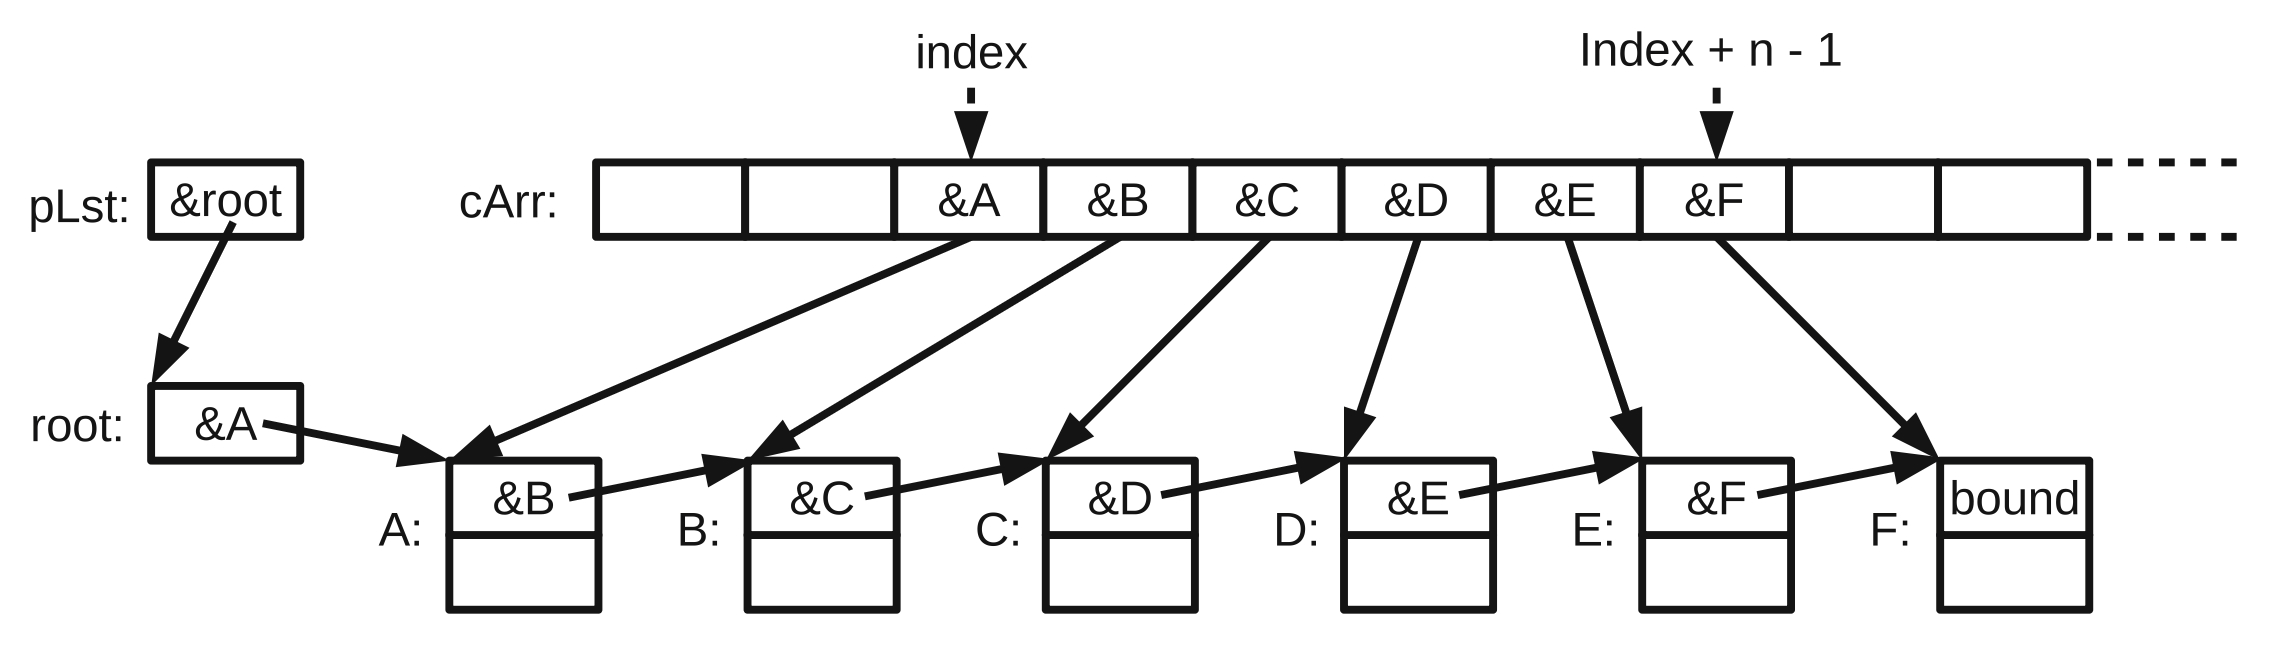
\includegraphics[width=\linewidth]{images/list-serialized}
    \caption{
        Vizualize serializace spojového seznamu. \\
        Převzato z článku Ghosts for Lists: A Critical Module of Contiki Verified in Frama\mbox{-}C~\cite{FCGhostsForLists}.
    }
    \label{fig:list-serialized}
\end{figure}

Serializace stromu, ve speciálním případě binární haldy
lze provést pomocí mapování prvků stromu do indexů pole dle následujícího vzorce.

Pokud je prvek na indexu $i$, pak levý potomek je na indexu $2i + 1$ a pravý potomek je na indexu $2i + 2$.
Rodičovský prvek je na indexu $\lfloor \frac{i - 1}{2} \rfloor$.
V binární haldě nemůže nastat situace s prázdným nepoužitým uzlem a pole se tedy vždy plní korektně
od nejnižšího indexu po nejvyšší.
Obecné stromy by s tímto principem nemohli být serializovány,
protože je možné, že některé uzly budou prázdné a nebudou mít žádného potomka.
Řešením se nabízí nepoužívat jednoduchou serializaci prvků stromu do pole,
ale používat rozšířenou strukturu v serializovaném poli, která nám určuje, zdali je
platný nebo ne.
Indexace prvků v poli by tímto přístupem byla zachována,
pouze program používající tuto strukturu by musel při každém přístupu na prvek stromu
zkontrolovat, zdali je prvek platný nebo ne.
O takto serializovaných stromech by bylo jednoduché provádět důkazy,
jelikož všechny prvky v poli jsou oddělené a tedy splňují podmínku oddělené paměti.
Predikáty popisující vlastnosti stromu by také obsahovali kontrolu, zdali je daný prvek v poli platný nebo ne.

Nevýhoda serializace obecných stormů do pole je ta, že řídké stromy budou zabírat
násobně více paměti než je potřeba.
V nejhorším případě, kdy by pomocí této metody byl zakódován strom obsahující řetězec \texttt{n} pravých uzlů,
by serailizované pole reprezentující tento strom mělo velikost $2^n - 1$ s $2^n - n$ neplatnými uzly.







%\section{Protipříklady}
%\label{sec:frama-c-counterexamples}

% TODO: pridat nedelitelnou mezeru tak, aby nebyly jedno-znaky na konci radku samy

%why3 config detect
%Found prover Alt-Ergo version 2.5.3, OK.
%Found prover Alt-Ergo version 2.5.3 (alternative: BV)
%Found prover Alt-Ergo version 2.5.3 (alternative: counterexamples)
%Found prover CVC4 version 1.8 (alternative: strings+counterexamples)
%Found prover CVC4 version 1.8 (alternative: strings)
%Found prover CVC4 version 1.8 (alternative: counterexamples)
%Found prover CVC4 version 1.8, OK.
%7 prover(s) added
%Save config to /home/parallels/.why3.conf


%2.3.3 Model Selection
%These options modify the underlying memory model that is used for computing weakest
%preconditions. See chapter 3 for details. Models are identified by a combination of selectors
%which are defined below:
%Selector Description
%Hoare Select Hoare memory model.
%Typed Select Typed memory model with limited casts.
%cast Select Typed memory model with unlimited casts (unsound).
%nocast Select Typed memory model with no casts.
%raw Disable the combination of memory models.
%var Combination of memory models based on variable analysis.
%ref Activate the detection of pointer variables used for reference passing style.
%caveat Caveat memory model (see 3.7).
%int Use machine integers when overflows and downcasts might occurs.
%nat Integer model without bounds (no overflow assumed).
%float Use floating-point operations.
%real Use mathematical reals instead of floating point.

